% Page 1
\begin{figure}[H]
    \centering
    \begin{subfigure}{\textwidth}
        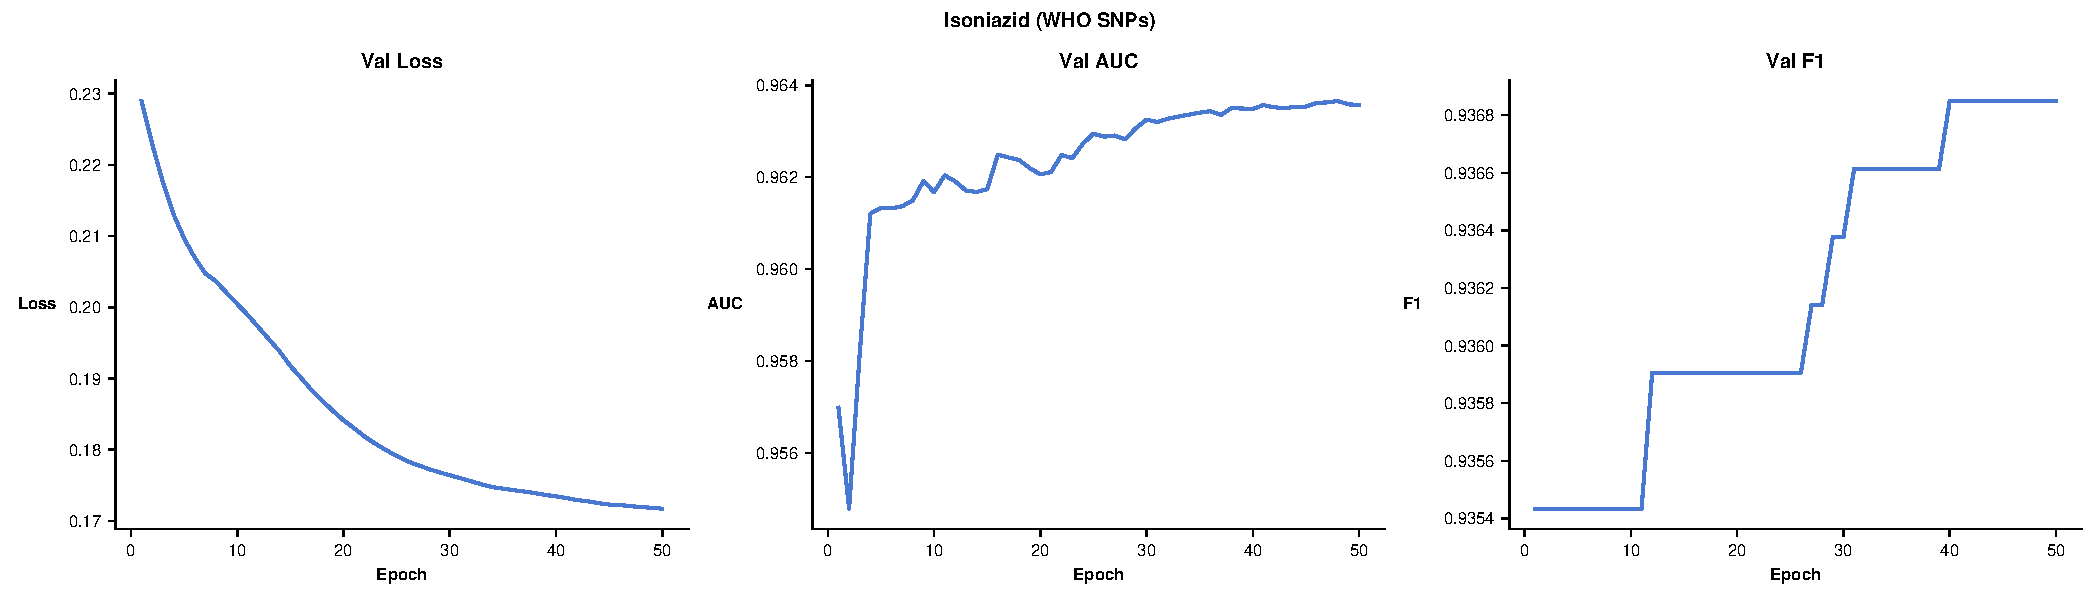
\includegraphics[width=\textwidth]{figures/who_isoniazid_learning_curves.pdf}
    \end{subfigure}
    \begin{subfigure}{\textwidth}
        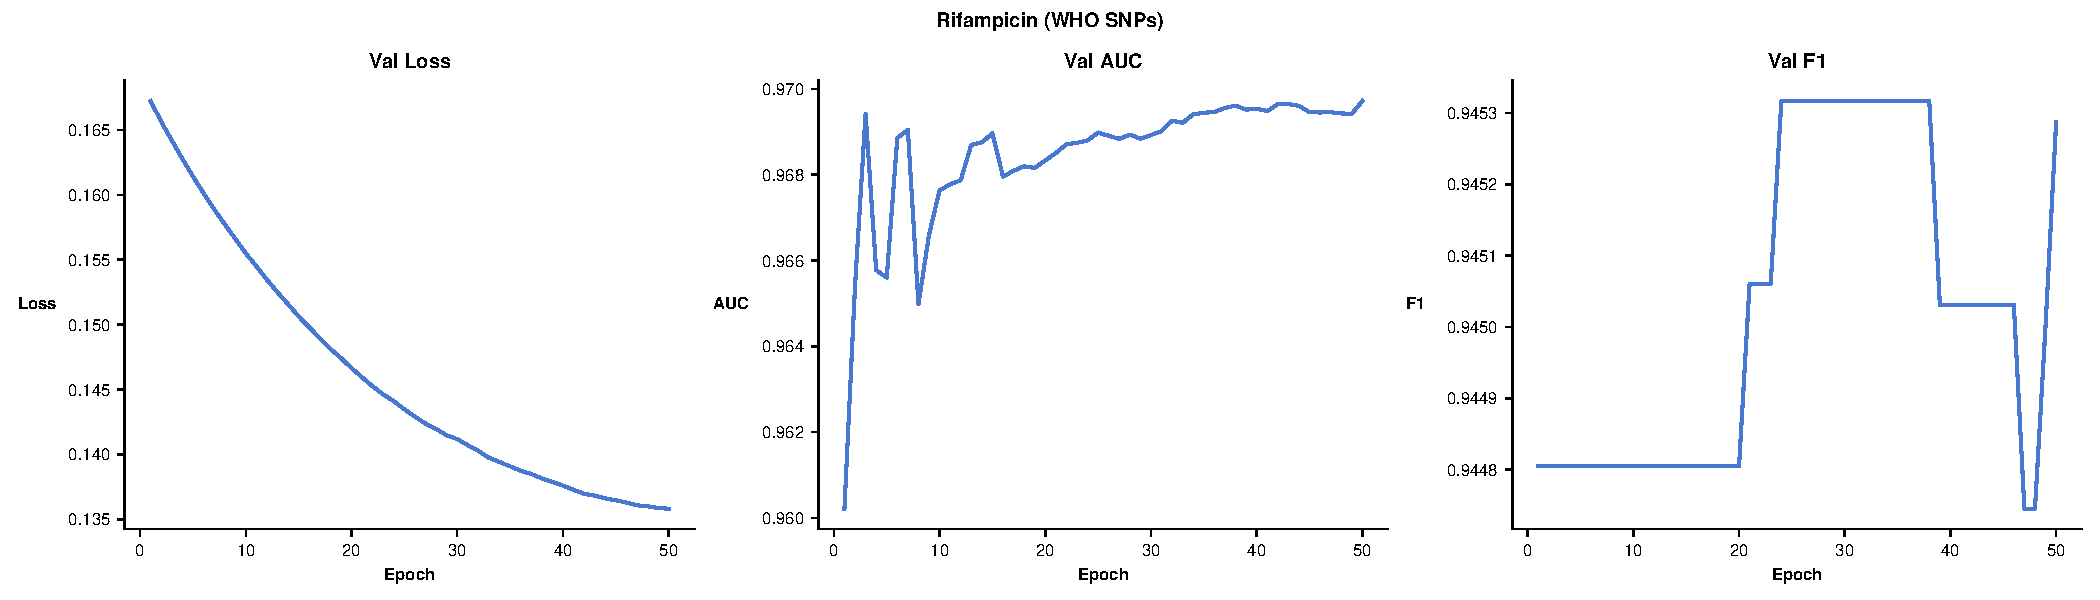
\includegraphics[width=\textwidth]{figures/who_rifampicin_learning_curves.pdf}
    \end{subfigure}
    \begin{subfigure}{\textwidth}
        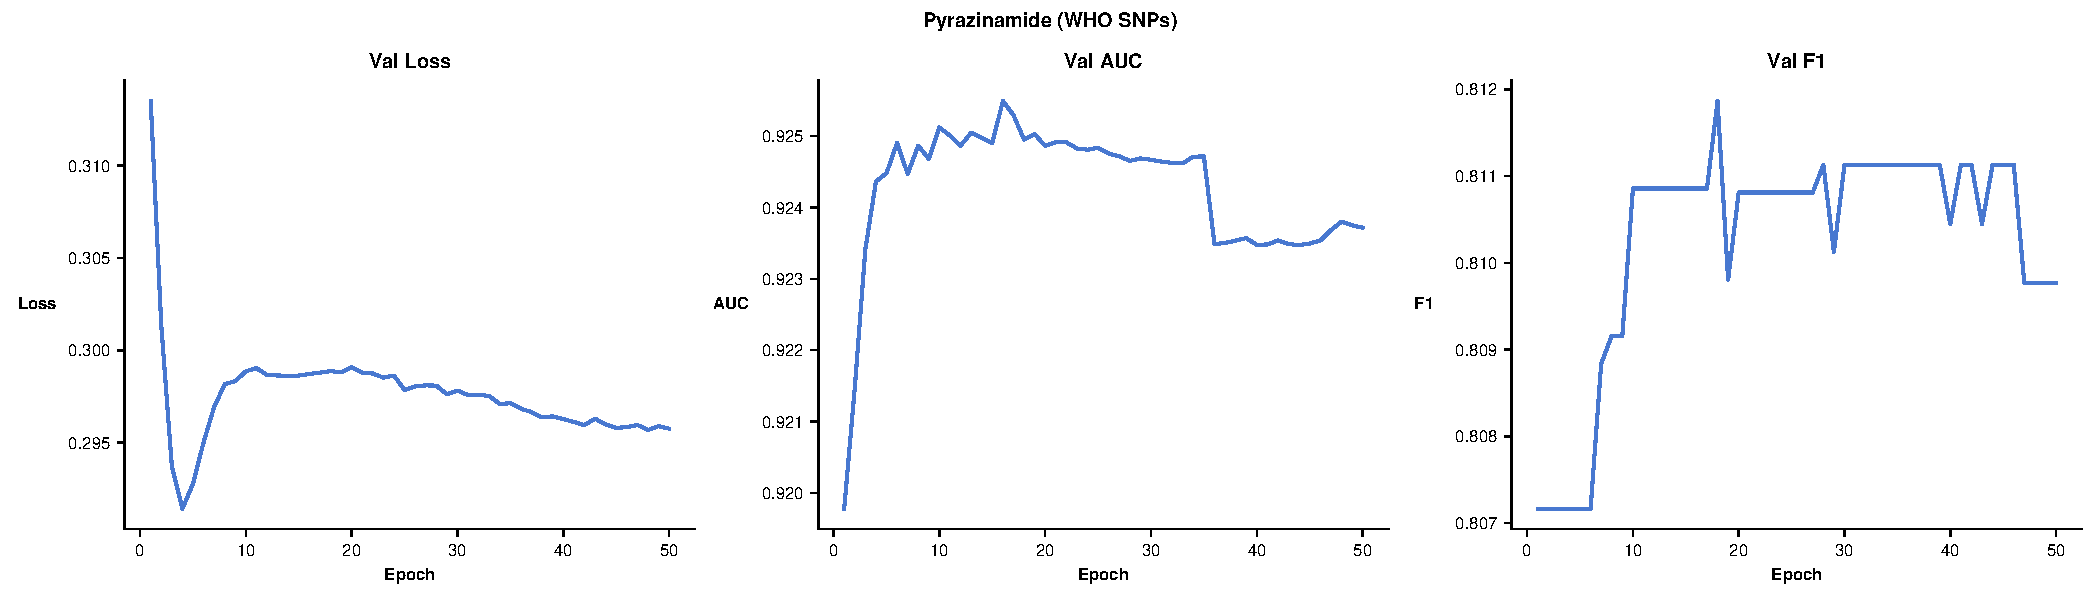
\includegraphics[width=\textwidth]{figures/who_pyrazinamide_learning_curves.pdf}
    \end{subfigure}
    \begin{subfigure}{\textwidth}
        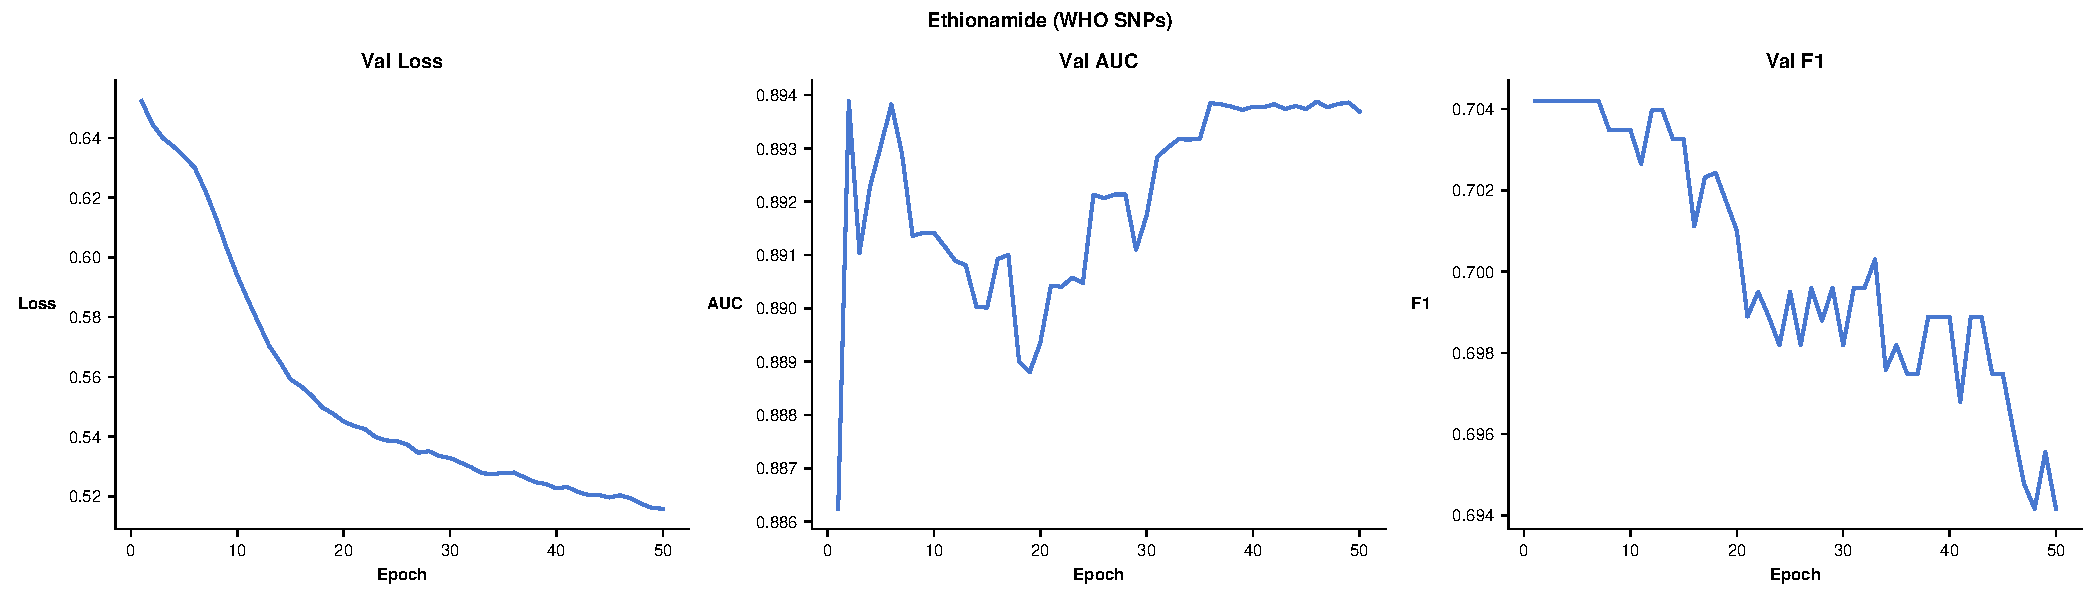
\includegraphics[width=\textwidth]{figures/who_ethionamide_learning_curves.pdf}
    \end{subfigure}
\end{figure}

\begin{figure}[H]
    \ContinuedFloat   % continues the same figure number
    \centering
    \begin{subfigure}{\textwidth}
        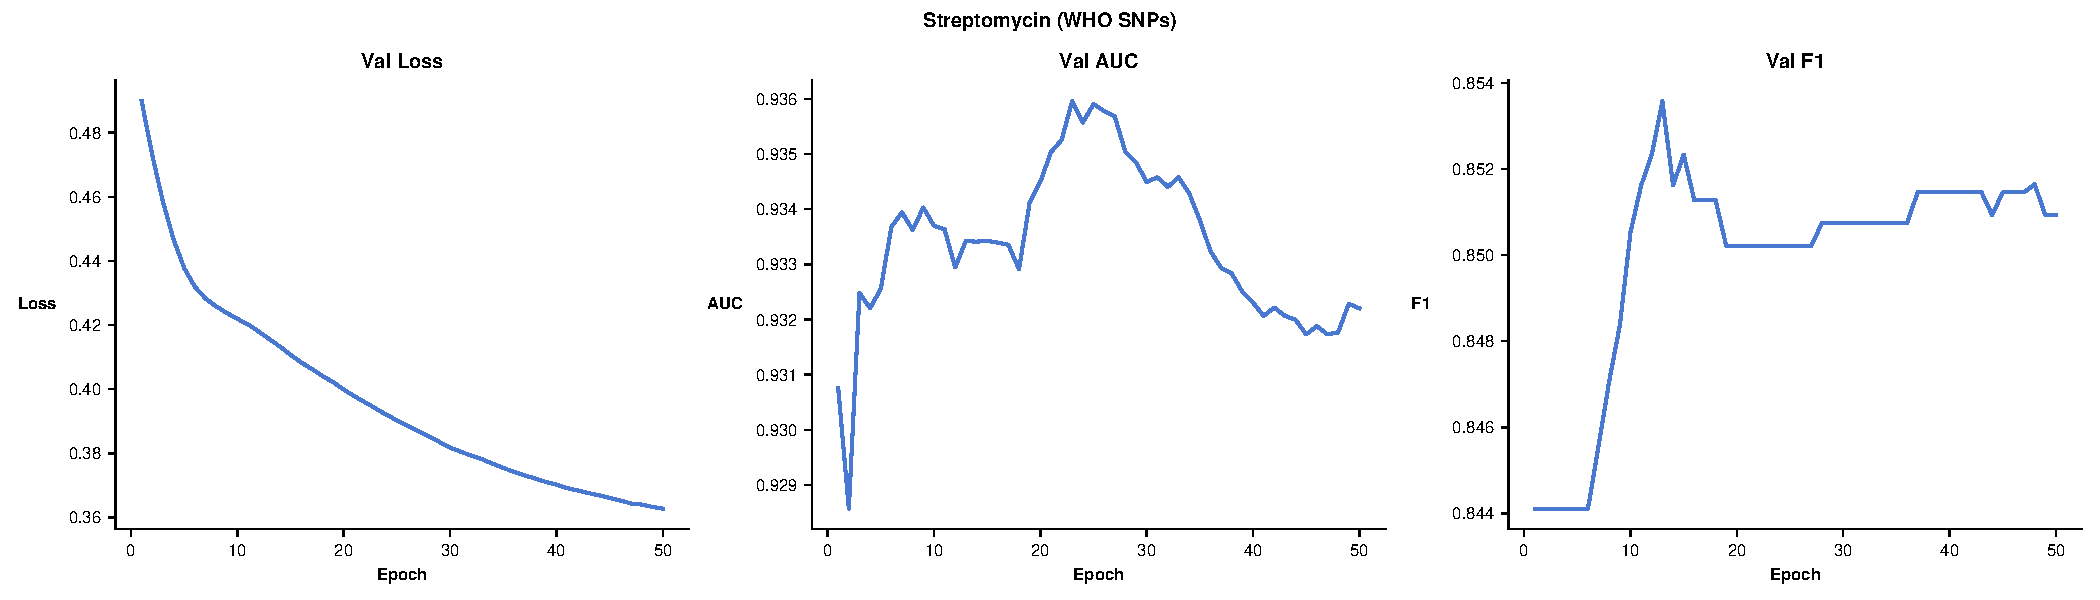
\includegraphics[width=\textwidth]{figures/who_streptomycin_learning_curves.pdf}
    \end{subfigure}
    \begin{subfigure}{\textwidth}
        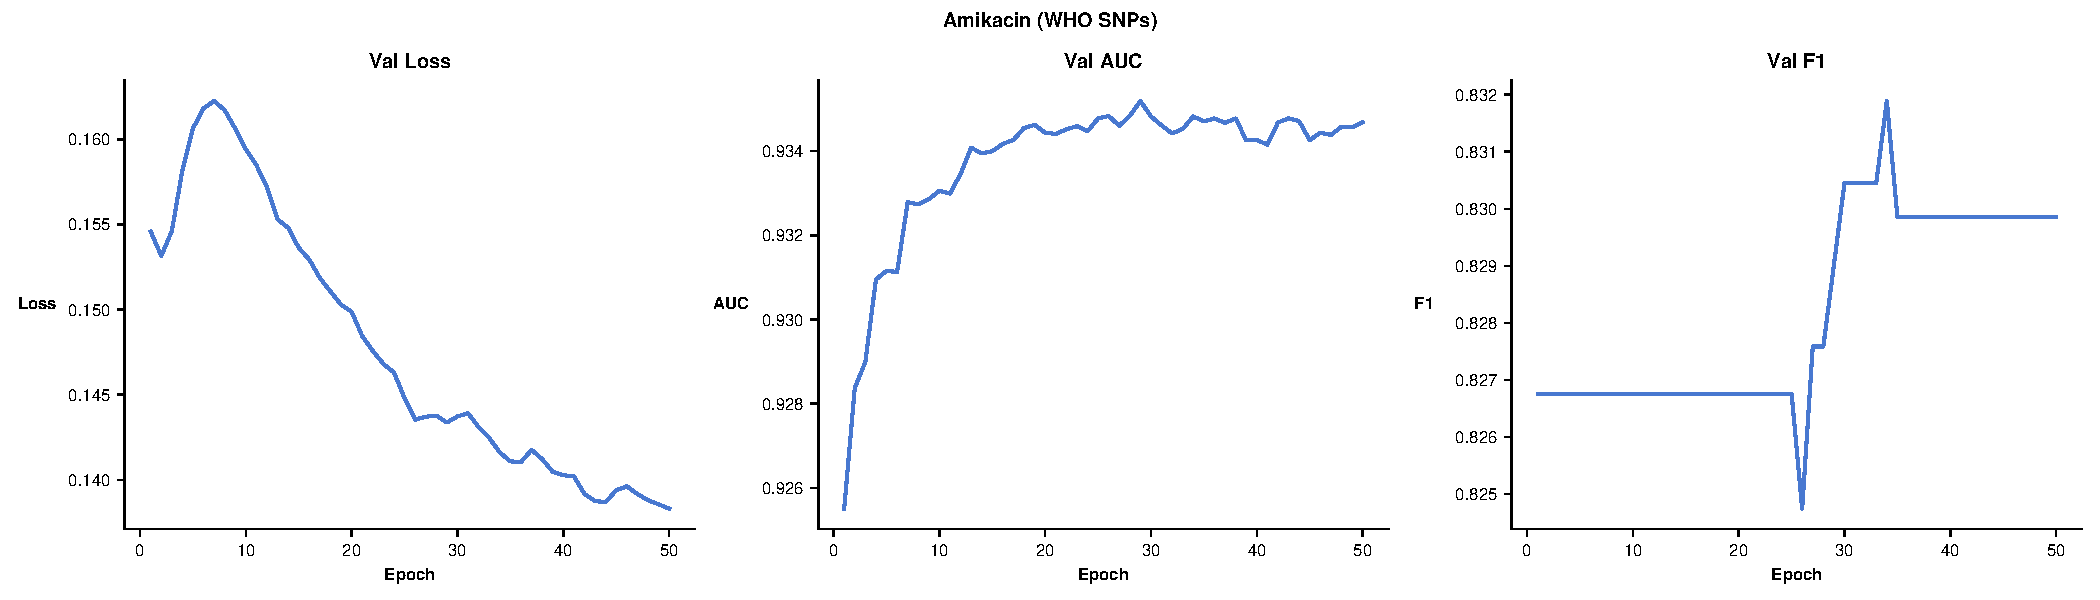
\includegraphics[width=\textwidth]{figures/who_amikacin_learning_curves.pdf}
    \end{subfigure}
    \begin{subfigure}{\textwidth}
        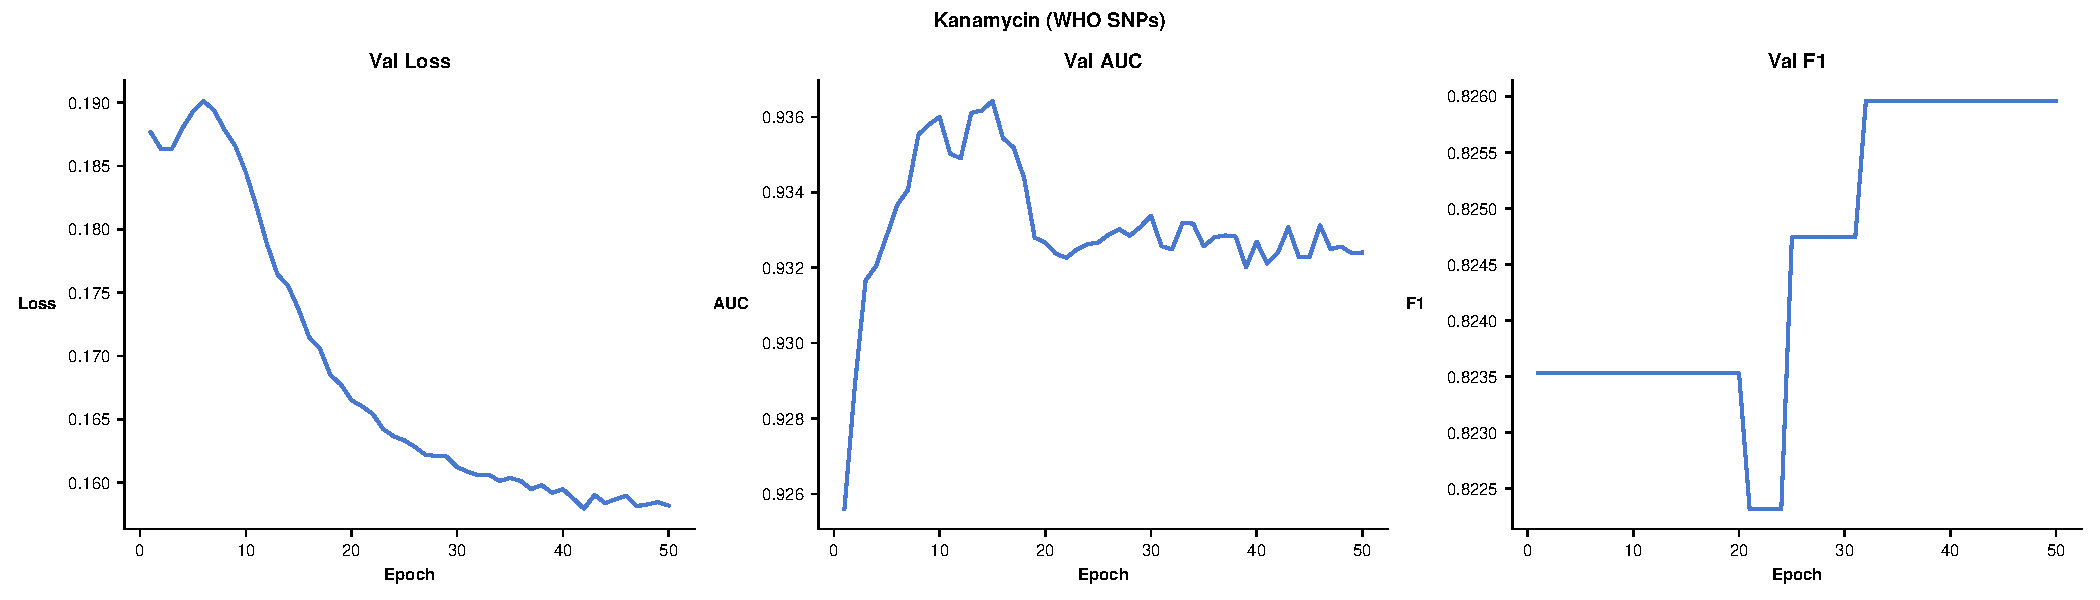
\includegraphics[width=\textwidth]{figures/who_kanamycin_learning_curves.pdf}
    \end{subfigure}
    \begin{subfigure}{\textwidth}
        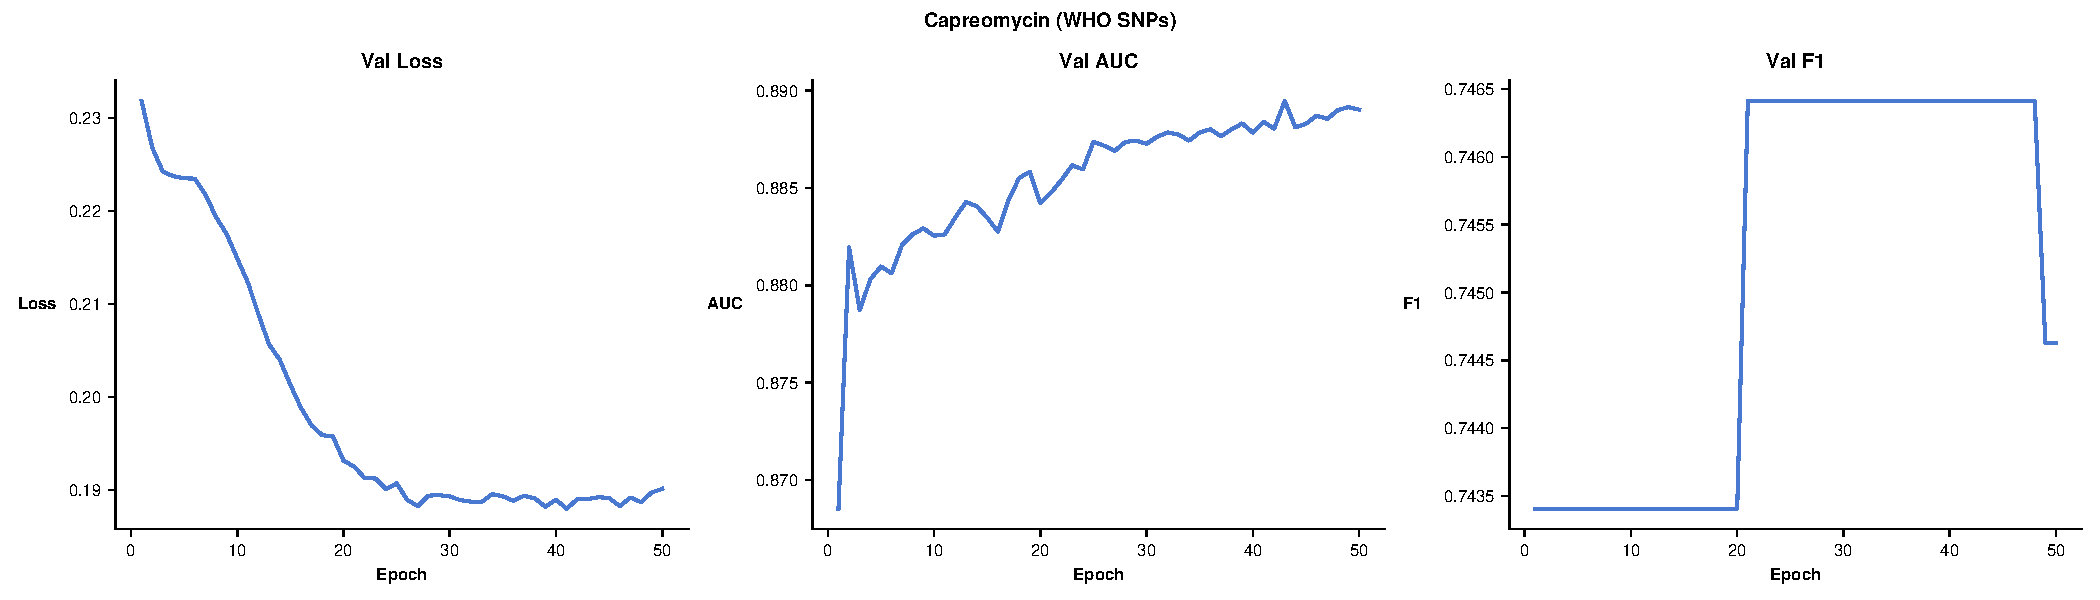
\includegraphics[width=\textwidth]{figures/who_capreomycin_learning_curves.pdf}
    \end{subfigure}
\end{figure}

\begin{figure}[H]
    \ContinuedFloat
    \centering
    \begin{subfigure}{\textwidth}
        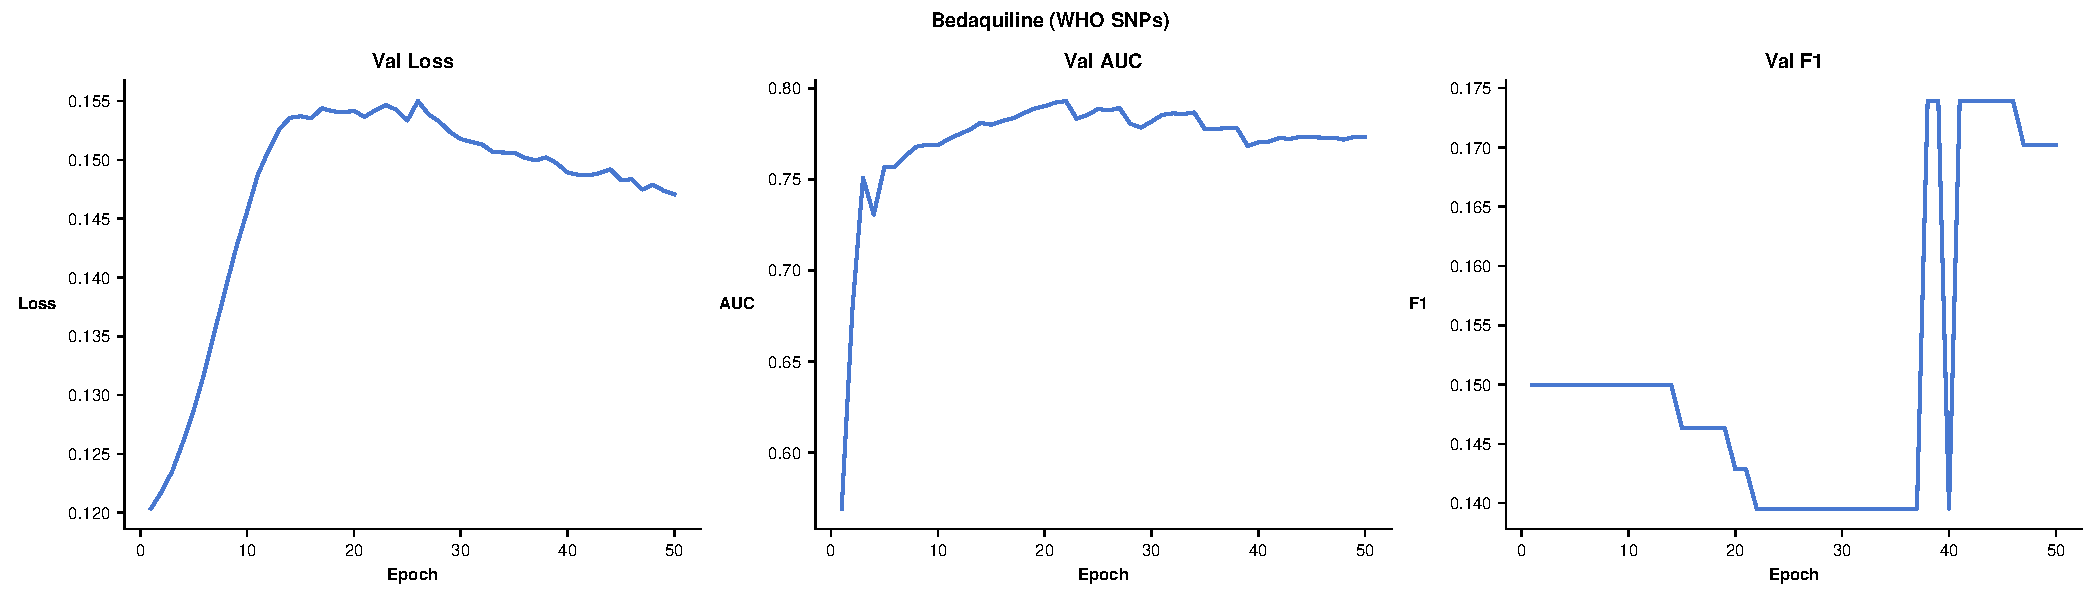
\includegraphics[width=\textwidth]{figures/who_bedaquiline_learning_curves.pdf}
    \end{subfigure}
    \begin{subfigure}{\textwidth}
        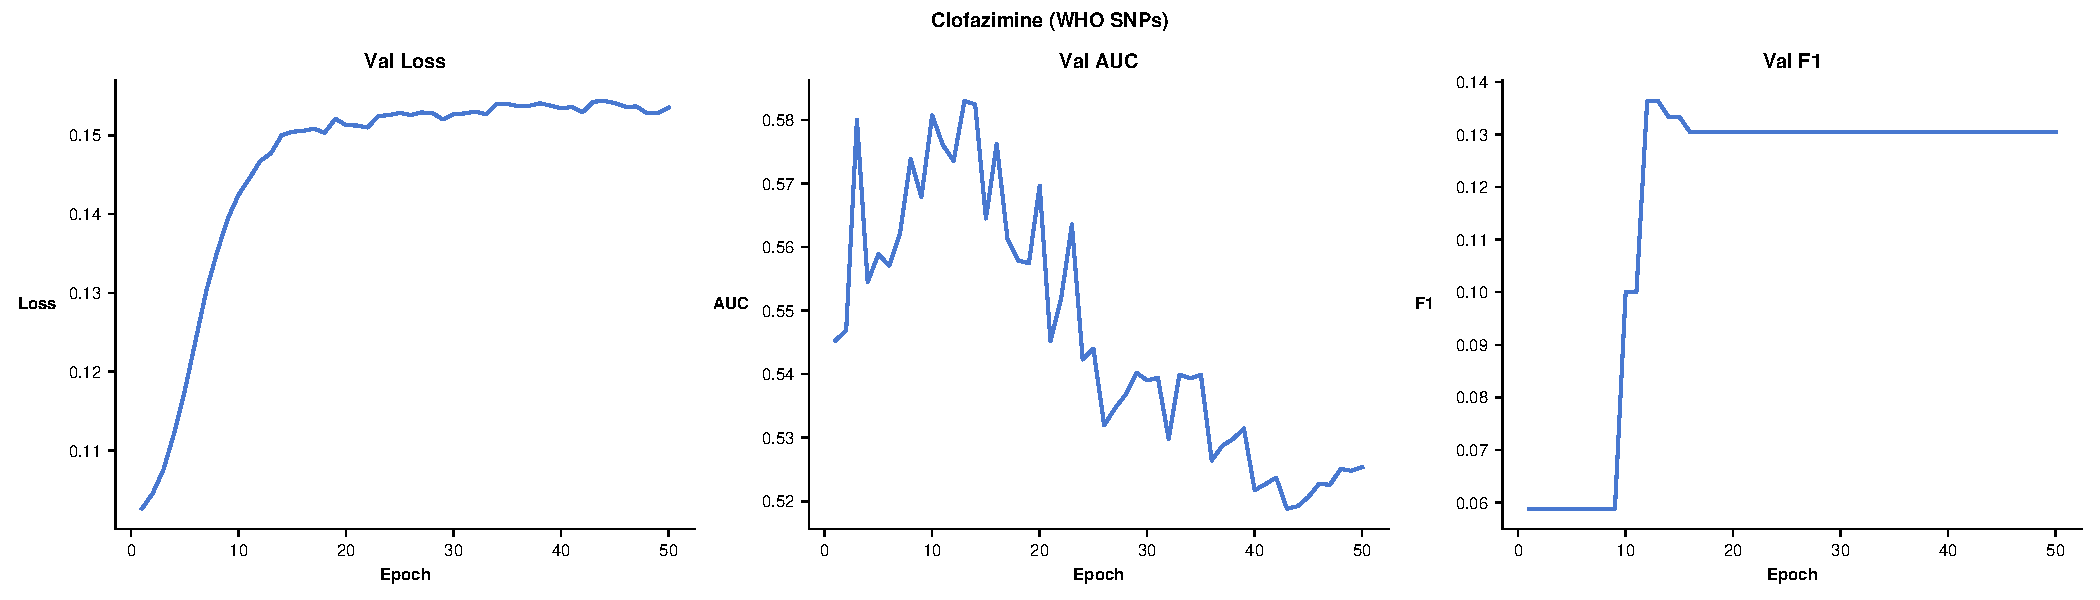
\includegraphics[width=\textwidth]{figures/who_clofazimine_learning_curves.pdf}
    \end{subfigure}
    \begin{subfigure}{\textwidth}
        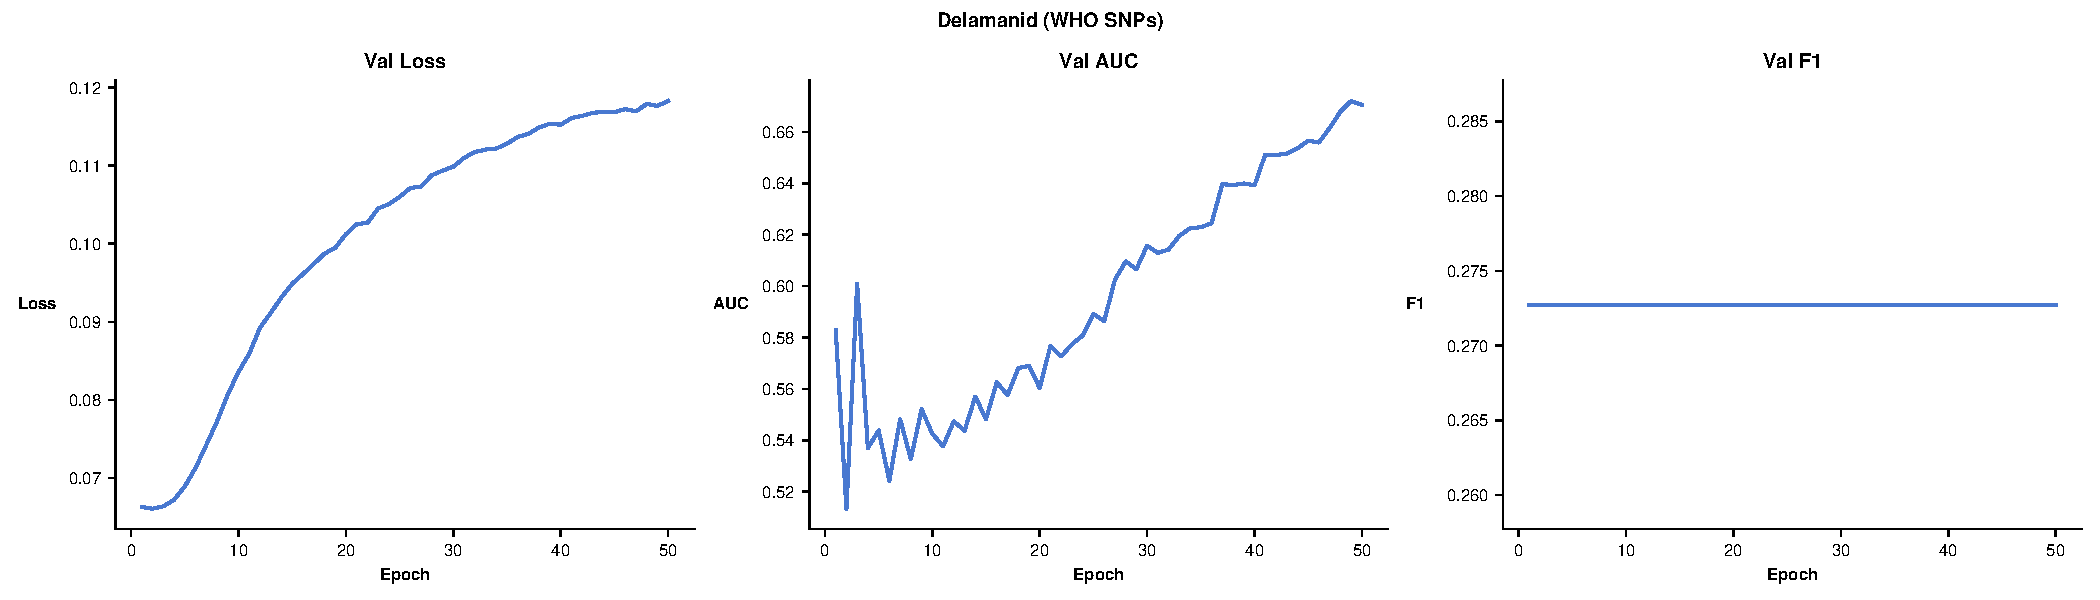
\includegraphics[width=\textwidth]{figures/who_delamanid_learning_curves.pdf}
    \end{subfigure}
    \begin{subfigure}{\textwidth}
        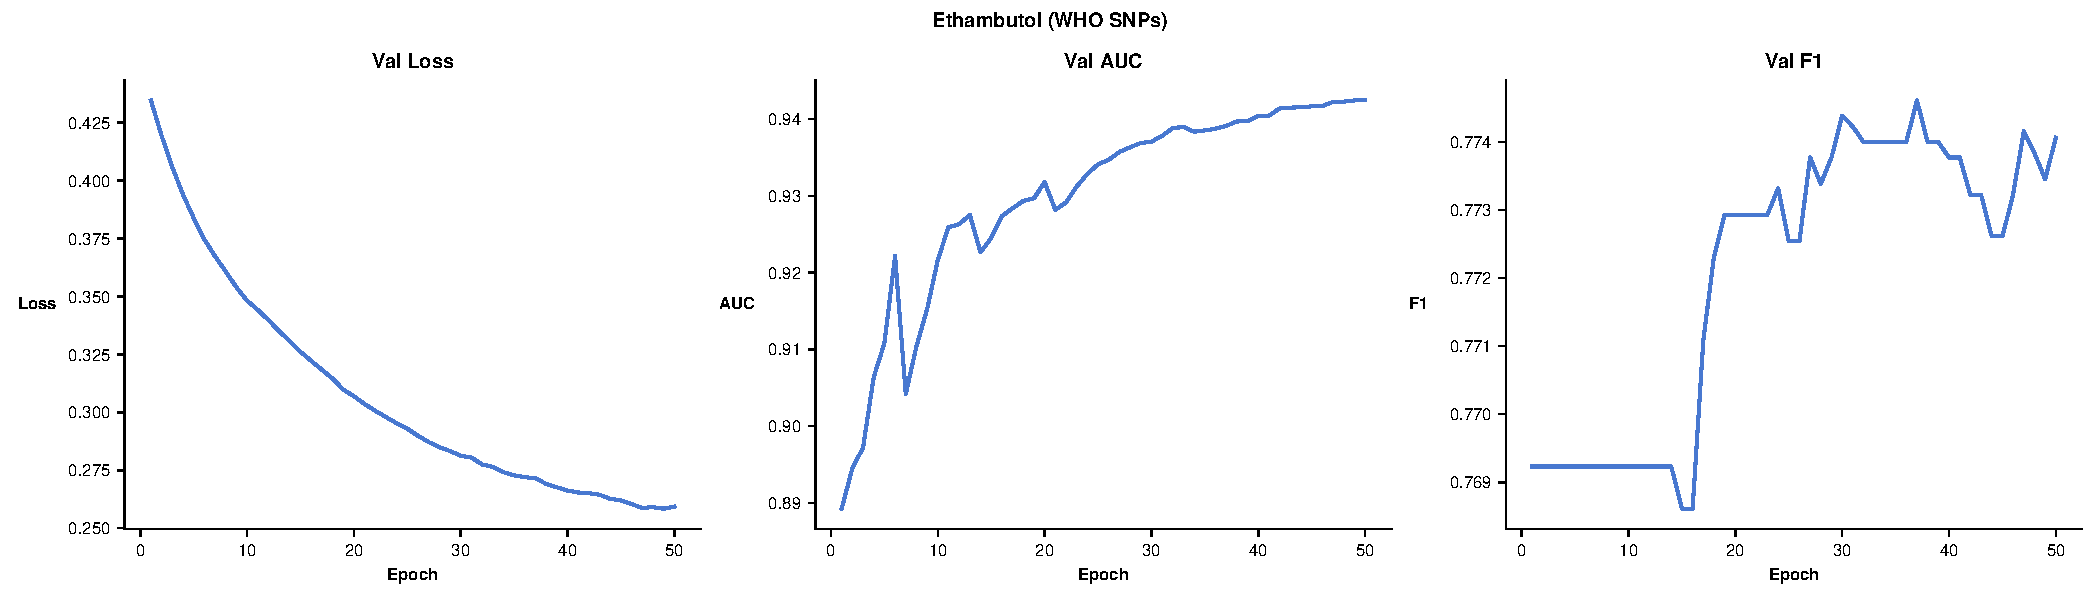
\includegraphics[width=\textwidth]{figures/who_ethambutol_learning_curves.pdf}
    \end{subfigure}
\end{figure}

\begin{figure}[H]
    \ContinuedFloat
    \centering
    \begin{subfigure}{\textwidth}
        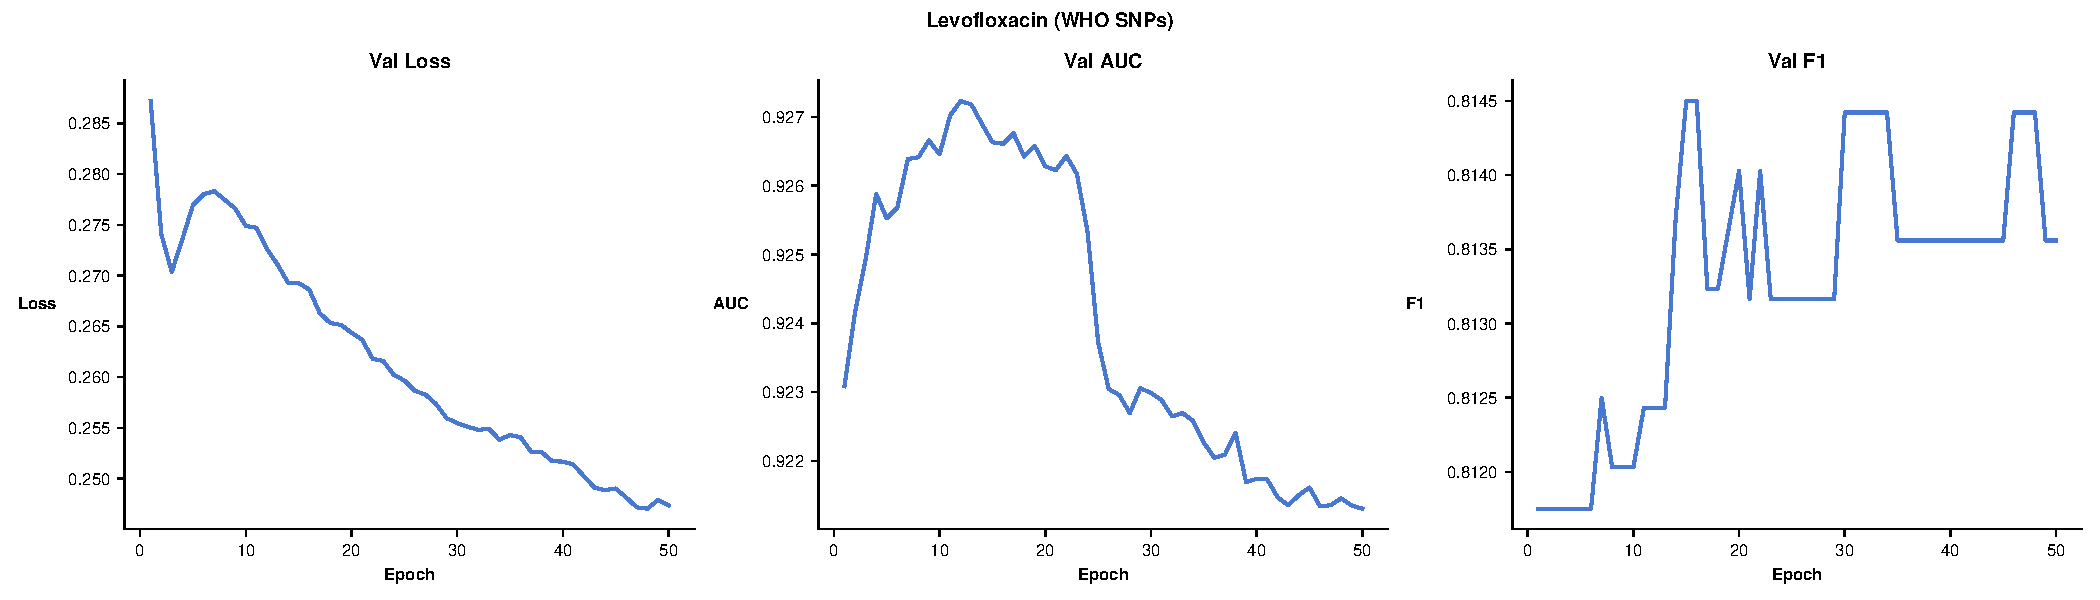
\includegraphics[width=\textwidth]{figures/who_levofloxacin_learning_curves.pdf}
    \end{subfigure}
    \begin{subfigure}{\textwidth}
        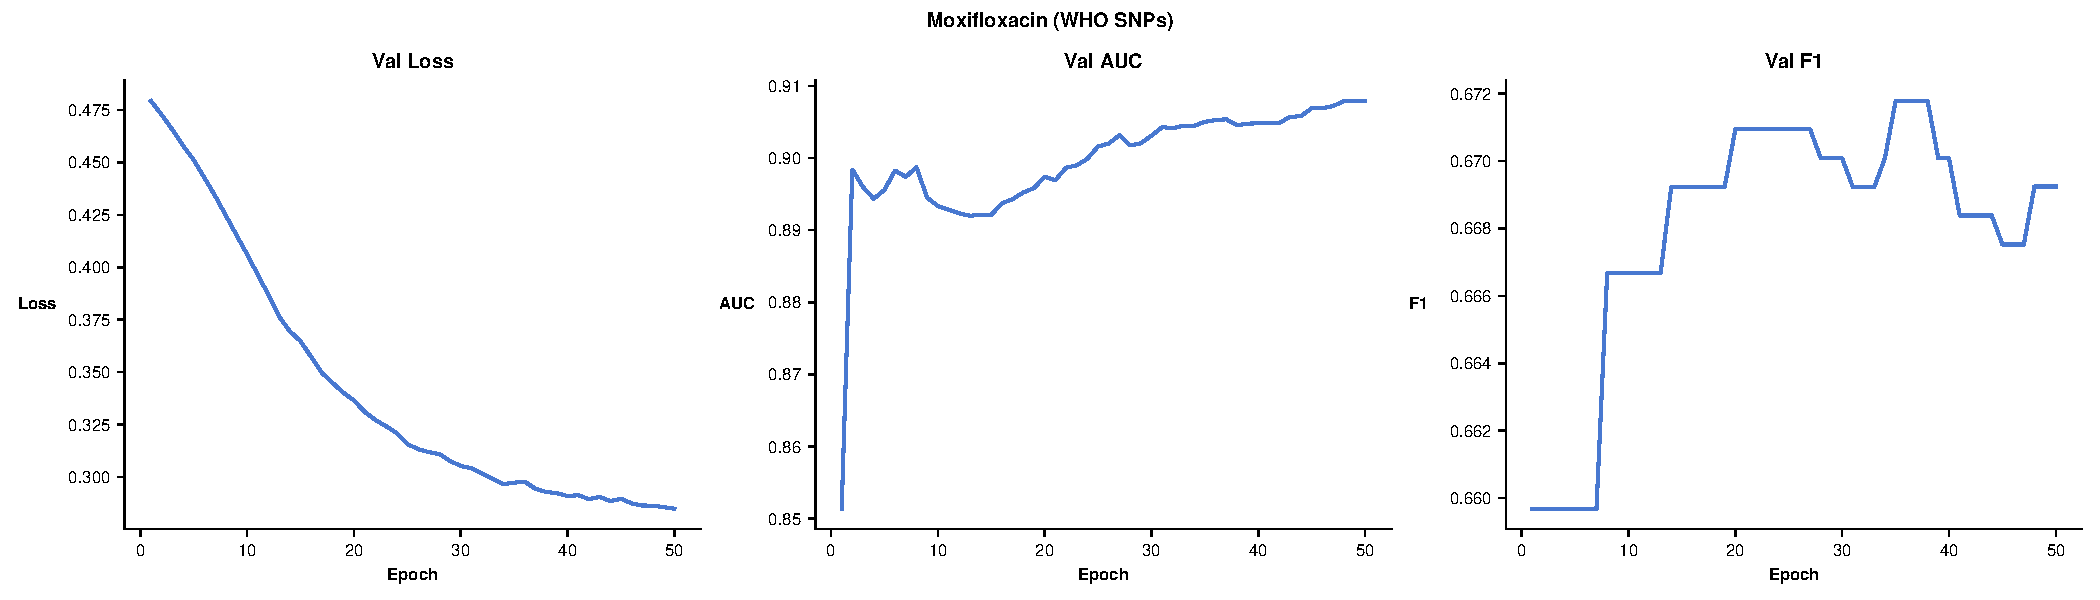
\includegraphics[width=\textwidth]{figures/who_moxifloxacin_learning_curves.pdf}
    \end{subfigure}
    \begin{subfigure}{\textwidth}
        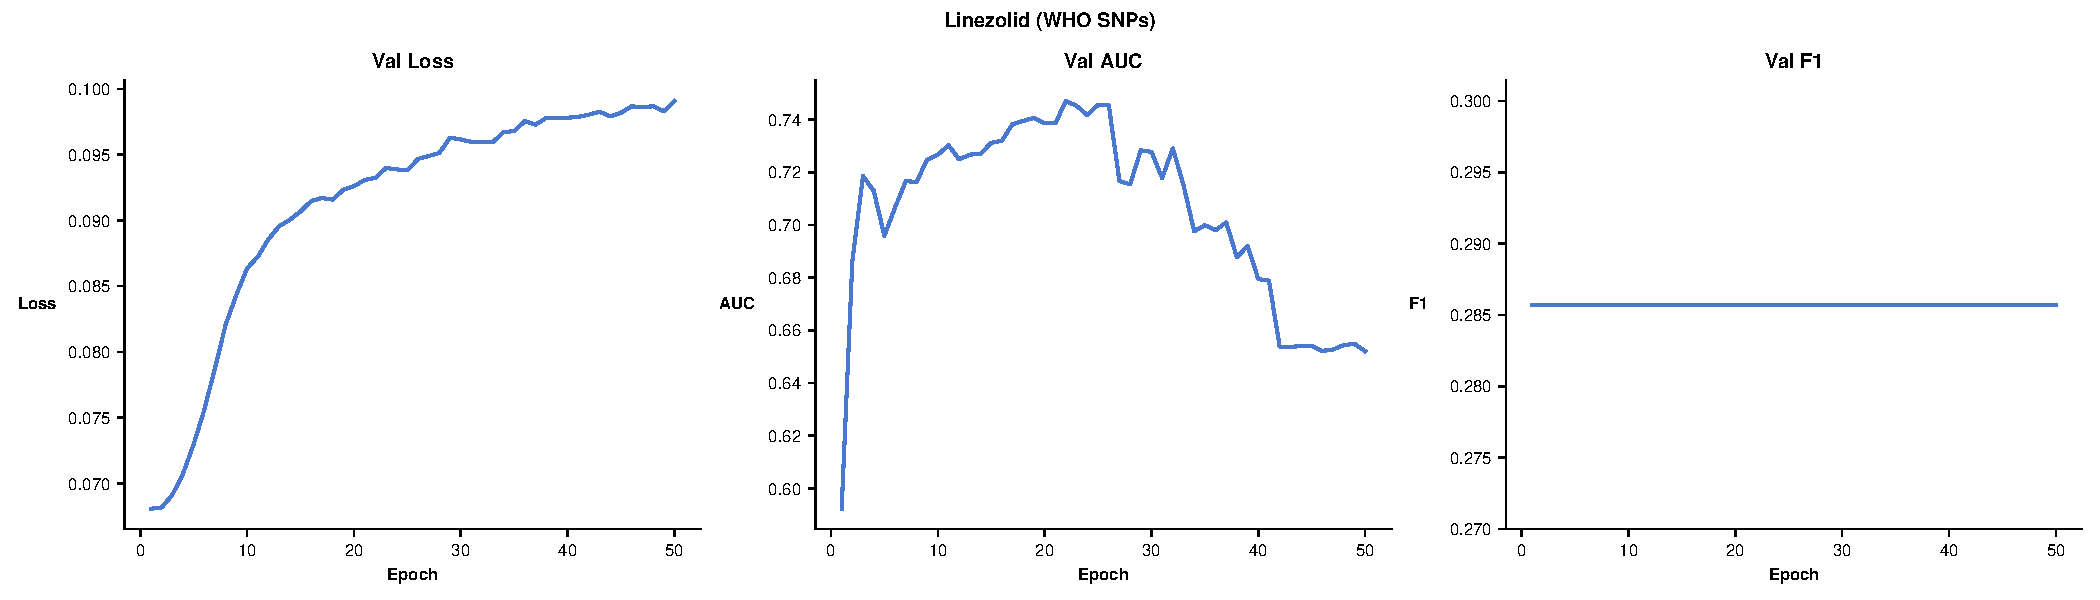
\includegraphics[width=\textwidth]{figures/who_linezolid_learning_curves.pdf}
    \end{subfigure}
    \caption{Model performance across all drugs}  % caption only on last block
    \label{fig:all_drugs}
\end{figure}
